%!TEX root = Main.tex
% System testing: words
\chapter{System Testing and Results} % (fold)
\label{cha:system_testing}

% Screenshots of data being sent and received (Logic)
% SystemVerilog simulations in ModelSim
% Hardware vs Software??? Roughly???
% Timing analysis / diagrams
% TODO: do some hardware analysis - how much current draw etc?

The testing methods and results are documented in this chapter, along with an analysis of the final design.  The two primary modules, described in the last chapter, were tested independently and then together, and will be presented here in the same manner.  A wide range of tools and techniques have been used to perform the testing, and to identify and fix errors encountered.


\section{Gaussian Distance Calculation Block} % (fold)
\label{sec:gaussian_distance_calculation_testing}
	There were several phases of development, and thus testing, of this block.  Initially, the full system was written and simulated in ModelSim, which supports SystemVerilog assertion based verification.  Each of the components of the design was built and tested separately, and then incrementally joined together and simulated as a whole.  Finally, the modules were tested in hardware -- first individually, and then as a full system.

	\subsection{Software Based Verification} % (fold)
	\label{sub:software_based_verification}
		A set of testbenches were developed for use within ModelSim, which tested each of the modules used by the system.  Most of the modules were fairly simple to simulate and verify, as the expected behaviour is generally constant and determinate.  For example, verifying the UART clock generator was a case of instantiating it, asserting the enable signal, and verifying the frequency of the output signals.  However, some modules and their testbenches deserve extra attention, as special methods were used to test them.
	
		The Gaussian Distance Pipe was initially tested by creating a testbench which provided the sequence of inputs that the GDP required, and then asserted that the correct score was provided.  Figure~\ref{fig:test_gdp} shows the correct operation of this module, with a set of test data being used as inputs to the module.  The correct results were found using the software GDP and the binary conversion software described in Section~\ref{sec:support_software}.

		\begin{figure}[tb]
			\begin{center}
				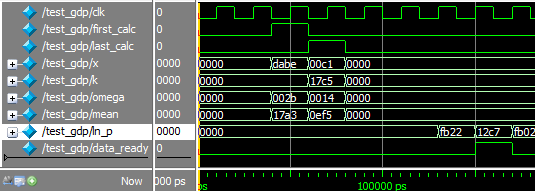
\includegraphics[width=\figwidth]{testbenches/gdp_wave.png}
			\end{center}
			\caption{GDP testbench waveform}
			\label{fig:test_gdp}
		\end{figure}
		
		The Gaussian Distance pipe controller testbench gives a new observation to the controller, and then watches as senone scores are produced by the module.  However, in order to test a large number of different inputs (which would result in different score outputs), a set of software utilities were written to automatically generate the testbench code.  This software made use of the HMM definition parser and a software version of the GDP that had already been created.  This allowed a very large number of senones to be tested in a matter of minutes, and determine how well the GDP pipe was working.

		Being able to easily test many senones was important because the use of fixed-point arithmetic inevitably causes numerical errors that vary with the operations and numbers being used.  The GDP may produce the correct result for one set of inputs, but another set of inputs may produce an erroneous result that was caused by the fixed-point number not having high enough precision.  In fact, in most cases, the least significant bits of the result were usually wrong.  Because of this, it was important to determine the distribution of the error magnitudes, in order to decide whether the number format needed changing.  Automatic testbench generation made this far easier, as testbenches could be created which automatically displayed which senone scores where wrong, and by how much.

		Other testbenches required a set of specific modules to emulate hardware that is otherwise non-existent in ModelSim, such as an external SRAM, or a UART connection.  Although these cannot model effects of real hardware, such as capacitative coupling, they are very useful for verifying that the SystemVerilog code works correctly.  Simulating and testing the UART module was done by creating two instances of the module, and cross-connecting their RX and TX pins.  This allowed both transmit and receive to be tested, and confirmed correct operation.  An example of this testbench running is shown in Figure~\ref{fig:test_uart}.  

		\begin{figure}[tb]
			\begin{center}
				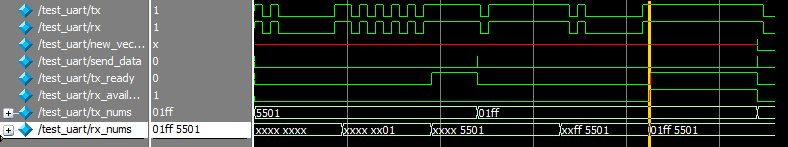
\includegraphics[width=\figwidth]{testbenches/uart_wave.png}
			\end{center}
			\caption{UART testbench waveform}
			\label{fig:test_uart}
		\end{figure}
	% subsection software_based_verification (end)

	\subsection{Hardware Based Verification} % (fold)
	\label{sub:hardware_based_verification}
		% TODO: Bus pirate, Saleae Logic
		After simulation, the UART module was finally verified by programming the FPGA with the UART module, and a simple controller which echoed back whatever it received.  An FTDI USB to serial cable connected the FPGA to a computer, so that the setup could be confirmed to work with a real UART connection.

		A custom SRAM module was built in order to test writing and reading values to the onboard SRAM chip, as it was a completely untested part of the board.

		Bus Pirate used to send stuff ....
	% subsection hardware_based_verification (end)

% section gaussian_distance_calculation_testing (end)


\section{Pre-Processing} % (fold)
\label{sec:pre_processing_testing}
	MFCCs not quite the same as HTK - further investigation needed to determine the reason.
	MFCC library slowwww.  
	The system works correctly otherwise.  
% section pre_processing_testing (end)


\section{Full system} % (fold)
\label{sec:full_system_testing}
	There were a few problems; a variety of tools were used to solve these.
% section full_system_testing (end)


\section{Analysis of Solution} % (fold)
\label{sec:analysis_of_solution}
% Move to testing / conclusions ??

	\subsection{The FPGA} % (fold)
	\label{sub:analysis_the_fpga}
		The FPGA used was very small, and the full required design could not fit on it.  In particular, the size of the model had to be reduced, so that each Senone had fewer than 25 components, and not all 7000 senones were processed.  This is mainly due to the small amount of onboard RAM on the FPGA, so the design would greatly benefit from having more RAM available.
	% subsection the_fpga (end)

	% The fixed point accuracy? 16 bit?

	% Evaluate the speed - how long did each cycle take.  How much time was added by adding another component? or another senone? Extrapolate?

	% The communication method (UART) is extremely slow and is the weakest point of the system.  It was used primarily for the ease of implementation, and because at this stage real-time operations are not required.  However, for this system to be realistically useful, a better communication method needs to be developed -- either a faster serial bus or some form of parallel connection.

	\subsection{The processor} % (fold)
	\label{sub:analysis_the_processor}
		% Weak points
		% The MFCC calculation has several problems.  The library used is slow and inefficient, and doesn't match the results given by HTK.
		% Do real sampling, not just reading wav files

	% subsection the_processor (end)

% section analysis_of_solution (end)

% chapter system_testing (end)